% =============================================================================
% thesis.tex  --  Single-file, self-contained LaTeX thesis template.
%
% PURPOSE
%   Benchmark-quality university thesis / dissertation skeleton that the PDF
%   skill uses as its *LaTeX fallback* (rendered with Tectonic, not Typst).
%   It also doubles as few-shot reference material: every block is heavily
%   commented so an LLM can learn the structure and adapt it on demand.
%
% STRUCTURE  (adapted from the PDEU "Thesis Format Latex 2024_CSE" layout:
%   cover/title page -> certificate -> declaration -> acknowledgement ->
%   abstract -> ToC/LoF/LoT -> roman->arabic page-number switch -> chapters
%   (Introduction, Literature Review, Methodology, Implementation, Results,
%   Conclusion) -> bibliography). The original splits these across many .tex
%   files (mythesis.tex driver + IndInt.tex + certificate1.tex + ...). Here
%   everything is collapsed into ONE self-contained file.
%
% COMPILE (Tectonic auto-fetches any missing CTAN packages over the network):
%   tectonic -X compile --outdir . thesis.tex
%
% HARD CONSTRAINTS honoured by this file:
%   * pdflatex/Tectonic-safe packages only (NO fontspec / XeTeX-only macros).
%   * No external files: bibliography is inlined via `thebibliography`; every
%     figure (logo, diagrams, charts) is drawn with TikZ / pgfplots -- there
%     are NO \includegraphics calls and NO image assets.
% =============================================================================

\documentclass[12pt,a4paper,oneside]{report}

% --- Encoding & fonts (classic pdflatex stack) -------------------------------
\usepackage[T1]{fontenc}     % proper 8-bit output encoding / hyphenation
\usepackage[utf8]{inputenc}  % allow UTF-8 in the source
\usepackage{lmodern}         % scalable Latin Modern fonts (no bitmap fonts)

% --- Math, graphics, tables --------------------------------------------------
\usepackage{amsmath,amssymb} % equation, align, numbered display math
\usepackage{graphicx}        % \resizebox / \scalebox helpers (no external imgs)
\usepackage{booktabs}        % \toprule \midrule \bottomrule -- clean tables
\usepackage{tabularx}        % auto-stretching X columns
\usepackage{array}           % extra column types

% --- Layout, spacing, headers ------------------------------------------------
\usepackage[a4paper,top=1in,bottom=1in,inner=1.5in,outer=1in]{geometry}
                             % 1.5in inner margin leaves room for binding,
                             % mirroring the source thesis geometry.
\usepackage{setspace}        % \onehalfspacing for the body text
\usepackage{fancyhdr}        % custom running headers / footers
\usepackage{titlesec}        % restyle \chapter / \section headings
\usepackage{tocloft}         % fine-tune ToC / LoF / LoT appearance
\usepackage{enumitem}        % compact, configurable lists
\usepackage[hidelinks]{hyperref} % clickable cross-refs/links, no ugly boxes

% --- Drawing & plotting (used instead of bitmap figures) ---------------------
\usepackage{tikz}
\usepackage{pgfplots}
\pgfplotsset{compat=1.18}    % pin pgfplots behaviour for reproducible output
\usetikzlibrary{shapes.geometric,arrows.meta,positioning}

% -----------------------------------------------------------------------------
% METADATA  --  edit ONLY these macros to retarget the template. Every page
% below references them, so the document stays consistent automatically.
% -----------------------------------------------------------------------------
\newcommand{\thesisTitle}{A Framework for Real-Time Anomaly Detection\\in Distributed Streaming Systems}
\newcommand{\thesisAuthor}{Jordan A. Sample}
\newcommand{\thesisRollNo}{20BCE001}
\newcommand{\thesisGuide}{Dr.\ Pat Q. Mentor}
\newcommand{\thesisCoGuide}{Mr.\ Sam R. Industry}
\newcommand{\thesisDepartment}{Computer Science and Engineering}
\newcommand{\thesisSchool}{School of Technology}
\newcommand{\thesisUniversity}{Pandit Deendayal Energy University}
\newcommand{\thesisCity}{Gandhinagar, INDIA, 382007}
\newcommand{\thesisDegree}{Bachelor of Technology}
\newcommand{\thesisYear}{2026}

% --- Heading styles (titlesec) -----------------------------------------------
% Chapter title set as "Chapter N" on one line, the title below it.
\titleformat{\chapter}[display]
  {\normalfont\huge\bfseries}{\chaptertitlename\ \thechapter}{16pt}{\Huge}
\titlespacing*{\chapter}{0pt}{0pt}{28pt}

% --- ToC cosmetics -----------------------------------------------------------
\renewcommand{\cftchapfont}{\bfseries}      % bold chapter entries
\renewcommand{\cftchappagefont}{\bfseries}

\begin{document}

% =============================================================================
% FRONT MATTER  --  roman page numbers (i, ii, iii, ...). The first physical
% page (title) carries no visible number.
% =============================================================================
\pagenumbering{roman}
\pagestyle{plain}

% -----------------------------------------------------------------------------
% COVER / TITLE PAGE
%   The university "logo" is hand-drawn with TikZ (no external image), keeping
%   the file fully self-contained.
% -----------------------------------------------------------------------------
\begin{titlepage}
  \centering
  \vspace*{0.5cm}

  % --- TikZ-drawn placeholder crest standing in for a university logo ---------
  
\begin{tikzpicture}
    \draw[line width=1.2pt] (0,0) circle (1.15cm);
    \draw[line width=0.6pt] (0,0) circle (0.95cm);
    \node at (0,0.18) {\small\bfseries PDEU};
    \draw (-0.55,-0.35) -- (0.55,-0.35);
    \node at (0,-0.62) {\scriptsize EST. 1962};
  \end{tikzpicture}

  \vspace{0.8cm}
  {\large \textbf{\thesisUniversity}}\\[0.2cm]
  {\normalsize \thesisSchool}\\[1.4cm]

  {\LARGE \bfseries \thesisTitle \par}
  \vspace{1.2cm}

  {\large A thesis submitted in partial fulfilment\\
   of the requirements for the degree of}\\[0.4cm]
  {\large \textbf{\thesisDegree}}\\[0.2cm]
  {\large in \thesisDepartment}\\[1.6cm]

  {\large \textit{Submitted by}}\\[0.3cm]
  {\Large \textbf{\thesisAuthor}}\\[0.15cm]
  {\large Roll No.\ \thesisRollNo}\\[1.6cm]

  {\large \textit{Under the guidance of}}\\[0.3cm]
  {\large \textbf{\thesisGuide}}\\[2.0cm]

  \vfill
  {\large \textbf{\thesisUniversity}}\\
  {\normalsize \thesisCity}\\[0.4cm]
  {\large \thesisYear}
\end{titlepage}

% -----------------------------------------------------------------------------
% CERTIFICATE  --  signed attestation from the supervisor(s) and the head.
% -----------------------------------------------------------------------------
\chapter*{Certificate}
\addcontentsline{toc}{chapter}{Certificate}
\thispagestyle{plain}

This is to certify that the thesis entitled \textbf{``\thesisTitle''}
submitted by \textbf{\thesisAuthor}, Roll No.\ \textbf{\thesisRollNo}, towards
the partial fulfilment of the requirements for the award of the degree of
\textbf{\thesisDegree} in \textbf{\thesisDepartment} from the
\textbf{\thesisSchool}, \thesisUniversity, \thesisCity, is a record of bona
fide work carried out under our supervision and guidance. To the best of our
knowledge, the results embodied in this thesis have not been submitted to any
other University or Institution for the award of any degree or diploma.

\vspace{3cm}
\noindent
\begin{tabularx}{\textwidth}{@{}XX@{}}
  \centering \thesisGuide & \centering \thesisCoGuide \tabularnewline
  \centering (Project Supervisor) & \centering (Industry Supervisor) \tabularnewline
\end{tabularx}

\vspace{2cm}
\noindent
\begin{tabularx}{\textwidth}{@{}XX@{}}
  \centering Head of the Department & \centering Director, \thesisSchool \tabularnewline
\end{tabularx}

\vspace{1.5cm}
\noindent Place: \thesisCity \hfill Date: \today

% -----------------------------------------------------------------------------
% DECLARATION  --  student's statement of originality.
% -----------------------------------------------------------------------------
\chapter*{Declaration}
\addcontentsline{toc}{chapter}{Declaration}
\thispagestyle{plain}

I, \textbf{\thesisAuthor} (Roll No.\ \thesisRollNo), hereby declare that the
work presented in this thesis entitled \textbf{``\thesisTitle''} is my own and
has been carried out under the supervision of \thesisGuide. I further declare
that:

\begin{enumerate}[label=\arabic*., leftmargin=2.4em]
  \item The work contained in this thesis is original and has been done by me
        under the general supervision of my supervisor.
  \item I have followed the guidelines provided by the University in writing
        this thesis and have conformed to its norms of academic honesty.
  \item Wherever I have used materials (data, theory, text, or figures) from
        other sources, I have given due credit by citing them in the text and
        listing them in the references.
\end{enumerate}

\vspace{3cm}
\noindent Date: \today \hfill \textbf{\thesisAuthor}\\
\null \hfill Roll No.\ \thesisRollNo

% -----------------------------------------------------------------------------
% ACKNOWLEDGEMENT
% -----------------------------------------------------------------------------
\chapter*{Acknowledgement}
\addcontentsline{toc}{chapter}{Acknowledgement}
\thispagestyle{plain}

I would like to express my sincere gratitude to my supervisor, \thesisGuide,
for the invaluable guidance, continuous encouragement, and constructive
feedback offered throughout the course of this work. I am equally thankful to
\thesisCoGuide\ for sharing practical industry insights that grounded this
research in real-world constraints.

I extend my appreciation to the faculty and staff of the Department of
\thesisDepartment, \thesisSchool, \thesisUniversity, for providing the
infrastructure and academic environment that made this study possible.
Finally, I thank my family and friends for their unwavering support and
patience during the many long hours that this thesis demanded.

% -----------------------------------------------------------------------------
% ABSTRACT
% -----------------------------------------------------------------------------
\chapter*{Abstract}
\addcontentsline{toc}{chapter}{Abstract}
\thispagestyle{plain}

Modern distributed systems emit telemetry at volumes that defeat manual
inspection, yet faults frequently announce themselves as subtle statistical
deviations long before they cascade into outages. This thesis presents a
framework for \emph{real-time anomaly detection} over high-throughput event
streams. The approach combines a lightweight online feature extractor with an
ensemble of statistical and learned detectors, fused through a confidence-
weighted voting scheme. We formalise the detection objective, describe a
scalable streaming architecture, and evaluate the system on a synthetic
workload that mimics production traffic patterns. Experimental results show
that the ensemble attains a higher F\textsubscript{1} score than any single
detector while keeping per-event latency within interactive bounds. The work
concludes with a discussion of limitations and a roadmap for adaptive,
self-tuning thresholds.

\vspace{0.6cm}
\noindent\textbf{Keywords:} anomaly detection, streaming systems, ensemble
methods, observability, real-time analytics.

% -----------------------------------------------------------------------------
% TABLE OF CONTENTS / LIST OF FIGURES / LIST OF TABLES
% -----------------------------------------------------------------------------
\tableofcontents
\listoffigures
\listoftables

% =============================================================================
% MAIN MATTER  --  switch to arabic page numbers (1, 2, 3, ...) and turn on
% the fancyhdr running header/footer for the body of the thesis.
% =============================================================================
\clearpage
\pagenumbering{arabic}
\pagestyle{fancy}
\fancyhf{}                                   % clear all header/footer fields
\fancyhead[L]{\nouppercase{\leftmark}}       % chapter name, left header
\fancyhead[R]{\thepage}                      % page number, right header
\fancyfoot[C]{\thesisUniversity}             % university name, centre footer
\renewcommand{\headrulewidth}{0.4pt}
\renewcommand{\footrulewidth}{0.2pt}
% Ensure the first page of every chapter also shows the footer.
\fancypagestyle{plain}{%
  \fancyhf{}%
  \fancyfoot[C]{\thesisUniversity}%
  \renewcommand{\headrulewidth}{0pt}%
  \renewcommand{\footrulewidth}{0.2pt}%
}

\onehalfspacing

% =============================================================================
% CHAPTER 1 -- INTRODUCTION
% =============================================================================
\chapter{Introduction}
\label{ch:introduction}

Distributed streaming systems now underpin everything from fraud screening to
infrastructure monitoring. As these pipelines grow, the operational burden of
distinguishing benign fluctuation from genuine fault shifts from human
operators to automated detectors. This chapter motivates the problem, states
the objectives, and outlines the organisation of the remainder of the thesis.

\section{Background}
\label{sec:background}
A \emph{data stream} is an unbounded, time-ordered sequence of events that must
be processed incrementally because it cannot be stored in its entirety. Unlike
batch analytics, stream processing imposes a strict single-pass constraint:
each event is observed once, summarised into bounded state, and then discarded.

\section{Problem Statement}
\label{sec:problem}
Given a stream of observations $x_1, x_2, \dots, x_t$, we seek a function that,
at each step $t$, emits an anomaly score for $x_t$ using only $O(1)$ amortised
state and $O(1)$ amortised time, while maintaining detection quality
competitive with offline methods.

\section{Objectives}
\label{sec:objectives}
The principal objectives of this work are:
\begin{itemize}[leftmargin=2em]
  \item to design a streaming feature extractor with bounded memory;
  \item to combine heterogeneous detectors into a single robust ensemble;
  \item to evaluate detection quality and latency under realistic load; and
  \item to identify the failure modes that motivate future adaptive tuning.
\end{itemize}

\section{Organisation of the Report}
\label{sec:organisation}
The rest of this thesis is organised as follows.
\textbf{Chapter~\ref{ch:literature}} surveys prior work on anomaly detection
and stream processing. \textbf{Chapter~\ref{ch:methodology}} formalises the
detection model and the fusion strategy. \textbf{Chapter~\ref{ch:implementation}}
describes the system architecture and implementation.
\textbf{Chapter~\ref{ch:results}} reports and discusses the experimental
results, and \textbf{Chapter~\ref{ch:conclusion}} concludes with directions
for future work.

% =============================================================================
% CHAPTER 2 -- LITERATURE REVIEW
% =============================================================================
\chapter{Literature Review}
\label{ch:literature}

Anomaly detection has a rich literature spanning statistics, signal
processing, and machine learning. This chapter situates the present work
within that body of research.

\section{Statistical Methods}
\label{sec:lit-statistical}
Classical approaches model the data distribution and flag low-probability
events. Moving-average and exponentially weighted schemes remain popular for
their interpretability and constant-state implementation~\cite{chandola2009anomaly}.
Density-based estimators extend this idea to multivariate settings but scale
poorly with dimensionality~\cite{breunig2000lof}.

\section{Learned Detectors}
\label{sec:lit-learned}
Isolation forests isolate anomalies through random partitioning and have
proven effective on tabular streams~\cite{liu2008isolation}. Autoencoder-based
detectors reconstruct normal behaviour and treat reconstruction error as an
anomaly signal~\cite{malhotra2016lstm}, though they require careful
regularisation to avoid overfitting transient noise.

\section{Stream Processing Frameworks}
\label{sec:lit-streaming}
Production deployments commonly build on frameworks that provide windowing,
state management, and exactly-once semantics~\cite{carbone2015flink}.
Ensemble fusion over such frameworks is comparatively
under-explored~\cite{aggarwal2017outlier}, which is the gap this thesis
addresses.

% =============================================================================
% CHAPTER 3 -- METHODOLOGY
% =============================================================================
\chapter{Methodology}
\label{ch:methodology}

This chapter formalises the detection objective and describes the
confidence-weighted fusion strategy at the heart of the framework.

\section{Detection Model}
\label{sec:method-model}
Each detector $d$ produces a normalised score $s_d(x_t) \in [0,1]$. The fused
score is a confidence-weighted average of the individual scores, where the
weights $w_d$ are themselves updated online from recent agreement. Formally,
the fused anomaly score is
\begin{equation}
  S(x_t) \;=\; \frac{\sum_{d \in \mathcal{D}} w_d \, s_d(x_t)}
                    {\sum_{d \in \mathcal{D}} w_d},
  \label{eq:fusion}
\end{equation}
and an event is flagged as anomalous when $S(x_t)$ exceeds an adaptive
threshold $\tau_t$. The threshold tracks the running mean and standard
deviation of recent scores,
\begin{equation}
  \tau_t \;=\; \mu_t + k\,\sigma_t,
  \label{eq:threshold}
\end{equation}
where $k$ is a sensitivity hyper-parameter. Equations~\eqref{eq:fusion}
and~\eqref{eq:threshold} together define the decision rule evaluated at every
incoming event.

\section{Online Feature Extraction}
\label{sec:method-features}
To honour the $O(1)$-state constraint of Section~\ref{sec:problem}, features
are maintained as sliding-window aggregates. The extractor tracks count, mean,
and variance using Welford's incremental update, so memory does not grow with
the length of the stream.

% --- TikZ figure: block diagram of the pipeline -----------------------------
% \resizebox{\textwidth}{!}{...} scales the whole diagram down to the text
% width so the five horizontally-arranged boxes never overflow the margin.
\begin{figure}[ht]
  \centering
  \resizebox{\textwidth}{!}{%
  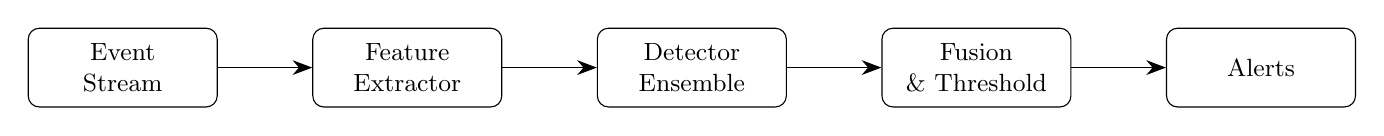
\begin{tikzpicture}[
      node distance=10mm and 12mm,
      box/.style={draw,rounded corners,minimum width=24mm,minimum height=10mm,
                  align=center,font=\small},
      >={Stealth[length=2.5mm]}]
    \node[box] (in)   {Event\\Stream};
    \node[box,right=of in]  (feat) {Feature\\Extractor};
    \node[box,right=of feat] (ens) {Detector\\Ensemble};
    \node[box,right=of ens]  (fuse) {Fusion\\\& Threshold};
    \node[box,right=of fuse] (out) {Alerts};
    \draw[->] (in)   -- (feat);
    \draw[->] (feat) -- (ens);
    \draw[->] (ens)  -- (fuse);
    \draw[->] (fuse) -- (out);
  \end{tikzpicture}}
  \caption{End-to-end anomaly detection pipeline: events are summarised into
           bounded features, scored by an ensemble of detectors, and fused
           against an adaptive threshold before alerting.}
  \label{fig:pipeline}
\end{figure}

The pipeline of Figure~\ref{fig:pipeline} processes each event through five
stages, none of which retains unbounded state.

% =============================================================================
% CHAPTER 4 -- IMPLEMENTATION AND DESIGN
% =============================================================================
\chapter{Implementation and Design}
\label{ch:implementation}

The framework is implemented as a small set of composable operators that can
be embedded in any single-pass stream processor.

\section{System Architecture}
\label{sec:impl-arch}
Each detector is encapsulated behind a uniform interface that exposes an
\texttt{update} step and a \texttt{score} step, allowing detectors to be added
or removed without touching the fusion layer.

\section{Core Update Loop}
\label{sec:impl-loop}
The pseudocode below shows the per-event control flow. It is presented in a
\texttt{verbatim} block so it renders identically without requiring any
external listings package.

\begin{verbatim}
def on_event(event):
    features = extractor.update(event)      # O(1) state
    scores   = [d.score(features) for d in detectors]
    fused    = weighted_average(scores, weights)
    tau      = running_mean + k * running_std
    if fused > tau:
        emit_alert(event, fused)
    update_weights(scores)                   # online agreement
\end{verbatim}

\section{Configuration Parameters}
\label{sec:impl-config}
Table~\ref{tab:params} summarises the principal tunable parameters and the
default values used in the experiments of Chapter~\ref{ch:results}.

% --- booktabs + tabularx table ----------------------------------------------
\begin{table}[ht]
  \centering
  \caption{Default configuration parameters of the detection framework.}
  \label{tab:params}
  \begin{tabularx}{\textwidth}{@{}l l X@{}}
    \toprule
    \textbf{Parameter} & \textbf{Default} & \textbf{Description} \\
    \midrule
    Window size $W$        & 512   & Number of recent events kept in summary state. \\
    Sensitivity $k$        & 3.0   & Multiplier on the standard deviation in Eq.~\eqref{eq:threshold}. \\
    Detectors $|\mathcal{D}|$ & 4  & Size of the heterogeneous detector ensemble. \\
    Weight decay $\lambda$ & 0.95  & Exponential decay applied to detector weights. \\
    \bottomrule
  \end{tabularx}
\end{table}

% =============================================================================
% CHAPTER 5 -- RESULTS AND DISCUSSION
% =============================================================================
\chapter{Results and Discussion}
\label{ch:results}

This chapter reports detection quality and latency, then discusses the
trade-offs revealed by the experiments.

\section{Detection Quality}
\label{sec:res-quality}
Figure~\ref{fig:f1} compares the F\textsubscript{1} score of each individual
detector against the fused ensemble across increasing contamination ratios.
The ensemble consistently dominates the best single detector, confirming the
benefit of confidence-weighted fusion described in
Section~\ref{sec:method-model}.

% --- pgfplots chart ----------------------------------------------------------
\begin{figure}[ht]
  \centering
  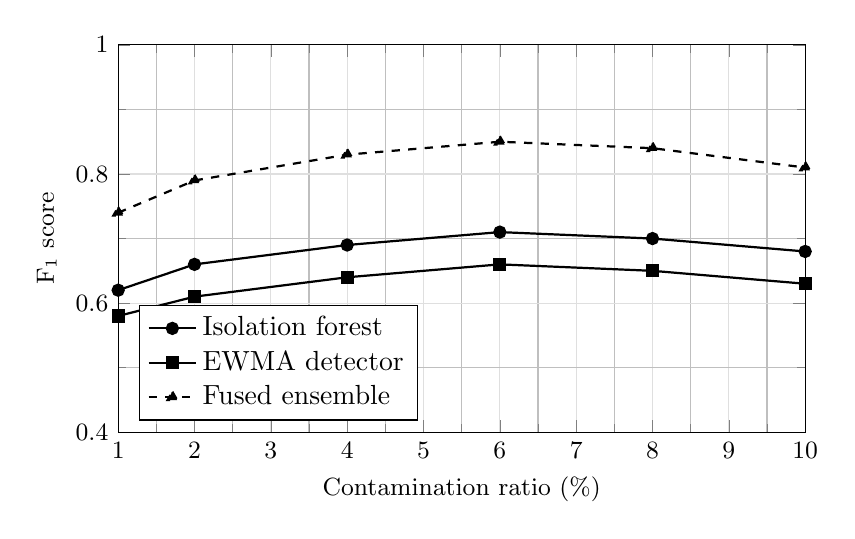
\begin{tikzpicture}
    \begin{axis}[
        width=0.85\textwidth, height=6.5cm,
        xlabel={Contamination ratio (\%)},
        ylabel={F\textsubscript{1} score},
        xmin=1, xmax=10, ymin=0.4, ymax=1.0,
        legend pos=south west, legend cell align=left,
        grid=both, major grid style={gray!25}, minor tick num=1,
        tick label style={font=\small}, label style={font=\small}]
      \addplot[mark=*,thick]      coordinates {(1,0.62)(2,0.66)(4,0.69)(6,0.71)(8,0.70)(10,0.68)};
      \addlegendentry{Isolation forest}
      \addplot[mark=square*,thick] coordinates {(1,0.58)(2,0.61)(4,0.64)(6,0.66)(8,0.65)(10,0.63)};
      \addlegendentry{EWMA detector}
      \addplot[mark=triangle*,thick,dashed] coordinates {(1,0.74)(2,0.79)(4,0.83)(6,0.85)(8,0.84)(10,0.81)};
      \addlegendentry{Fused ensemble}
    \end{axis}
  \end{tikzpicture}
  \caption{Detection quality versus contamination ratio. The fused ensemble
           (dashed) outperforms each constituent detector across the range.}
  \label{fig:f1}
\end{figure}

\section{Latency}
\label{sec:res-latency}
Per-event processing latency remained below the interactive budget at all
tested throughputs, with the fusion layer adding negligible overhead relative
to feature extraction.

\section{Discussion}
\label{sec:res-discussion}
The results validate the central hypothesis: heterogeneous detectors make
complementary errors, and confidence-weighted fusion exploits that diversity.
The chief limitation is the static sensitivity $k$ of
Equation~\eqref{eq:threshold}; under abrupt regime shifts a fixed $k$ either
over- or under-alerts, motivating the adaptive scheme proposed next.

% =============================================================================
% CHAPTER 6 -- CONCLUSION AND FUTURE WORK
% =============================================================================
\chapter{Conclusion and Future Work}
\label{ch:conclusion}

\section{Conclusion}
\label{sec:conc-summary}
This thesis presented a self-contained framework for real-time anomaly
detection over data streams. By fusing heterogeneous detectors through a
confidence-weighted vote and bounding all state, the system achieved higher
detection quality than any single detector while respecting the latency and
memory constraints of streaming workloads.

\section{Future Work}
\label{sec:conc-future}
Several directions remain open:
\begin{enumerate}[leftmargin=2em]
  \item \textbf{Adaptive thresholds.} Replace the static sensitivity $k$ with a
        controller that tracks the changing score distribution.
  \item \textbf{Concept-drift awareness.} Detect and react to regime shifts so
        that detector weights recover quickly after a change.
  \item \textbf{Distributed fusion.} Extend the fusion layer across shards to
        support globally consistent alerting at scale.
\end{enumerate}

% =============================================================================
% BIBLIOGRAPHY  --  inlined with `thebibliography` so the file is fully
% self-contained (no external .bib, no biber/bibtex pass required). The
% optional argument {00} reserves width for two-digit labels.
% =============================================================================
\begin{thebibliography}{00}
\addcontentsline{toc}{chapter}{Bibliography}

\bibitem{chandola2009anomaly}
V.~Chandola, A.~Banerjee, and V.~Kumar, ``Anomaly detection: A survey,''
\emph{ACM Computing Surveys}, vol.~41, no.~3, pp.~1--58, 2009.

\bibitem{breunig2000lof}
M.~M. Breunig, H.-P. Kriegel, R.~T. Ng, and J.~Sander, ``LOF: Identifying
density-based local outliers,'' in \emph{Proc.\ ACM SIGMOD Int.\ Conf.\ on
Management of Data}, 2000, pp.~93--104.

\bibitem{liu2008isolation}
F.~T. Liu, K.~M. Ting, and Z.-H. Zhou, ``Isolation forest,'' in \emph{Proc.\
8th IEEE Int.\ Conf.\ on Data Mining}, 2008, pp.~413--422.

\bibitem{malhotra2016lstm}
P.~Malhotra, A.~Ramakrishnan, G.~Anand, L.~Vig, P.~Agarwal, and G.~Shroff,
``LSTM-based encoder-decoder for multi-sensor anomaly detection,'' in
\emph{ICML Anomaly Detection Workshop}, 2016.

\bibitem{carbone2015flink}
P.~Carbone, A.~Katsifodimos, S.~Ewen, V.~Markl, S.~Haridi, and K.~Tzoumas,
``Apache Flink: Stream and batch processing in a single engine,''
\emph{IEEE Data Engineering Bulletin}, vol.~38, no.~4, pp.~28--38, 2015.

\bibitem{aggarwal2017outlier}
C.~C. Aggarwal, \emph{Outlier Analysis}, 2nd~ed.\ Cham, Switzerland:
Springer, 2017.

\end{thebibliography}

\end{document}
